\chapter{The Prevalence and Impact of Cheating in Online Multiplayer Games}

Building upon the historical and sociotechnical evolution of video game cheating, from its origins in debugging tools to its current manifestation as a sophisticated, commercialized industry, we now examine its pervasive impact on contemporary gaming communities and market dynamics.

Cheating in online multiplayer games constitutes an escalating systemic threat that undermines fairness, erodes player trust, and destabilizes gaming ecosystems. This chapter delves into the multifaceted consequences of cheating, with particular emphasis on the evolving landscape surrounding \textit{Counter-Strike 2} (CS2), and argues that addressing this issue demands an integrated response encompassing technical, legal, and social countermeasures.

As competitive online titles continue to thrive, especially those featuring ranked ladders, esports ecosystems, and in-game economies, the incentives to obtain unfair advantages intensify. This dynamic perpetuates a relentless arms race between cheat developers and game studios, necessitating not only robust technological defenses but also a comprehensive understanding of the socio-economic impacts of cheating.

\section{Cheating as a Critical Threat to Player Retention}

Cheating is not merely a minor inconvenience; it stands as a significant factor contributing to player attrition and dissatisfaction. A global survey conducted by Irdeto revealed that 60\% of players reported a negative impact on their gaming experience due to cheating, and 77\% indicated they would discontinue playing a game if cheating became widespread \parencite{irdeto2018global}.

\begin{table}[H]
  \centering
  \caption{Survey Results on Cheating in Online Games (Irdeto, 2018)}
  \label{tab:irdeto-survey}
  \begin{tabular}{|p{10cm}|c|}
  \hline
  \textbf{Survey Statement} & \textbf{Percentage of Respondents} \\
  \hline
  Experienced negative impact due to cheating & 60\% \\
  Would stop playing a game because of cheaters & 77\% \\
  Support permanent bans for cheaters & 69\% \\
  Believe developers are not doing enough & 55\% \\
  \hline
  \end{tabular}
\end{table}

These findings underscore that cheating not only generates immediate frustration but also carries long-term economic implications. Since player engagement drives monetization through mechanisms such as battle passes, cosmetic sales, and advertising, a decline in player retention fueled by cheating poses a direct threat to publishers' revenue streams.

Ultimately, when players perceive ranked systems, matchmaking, or competitive outcomes as compromised, they are likely to migrate toward alternative titles, thereby undermining the sustainability and vitality of the gaming community.

\section{Case Study: Cheating in \textit{Counter-Strike 2}}

\textit{Counter-Strike 2} (CS2) stands as a prominent example of modern cheating dynamics within competitive first-person shooter games. Its expansive player base and vibrant esports scene make it both an attractive target for cheat developers and a critical testing ground for anti-cheat innovations.

To contextualize the scale of CS2's ecosystem, Figure~\ref{fig:cs2-playerbase} illustrates the evolution of its player base from January 2024 to April 2025, based on data from SteamCharts:

\begin{figure}[H]
  \centering
  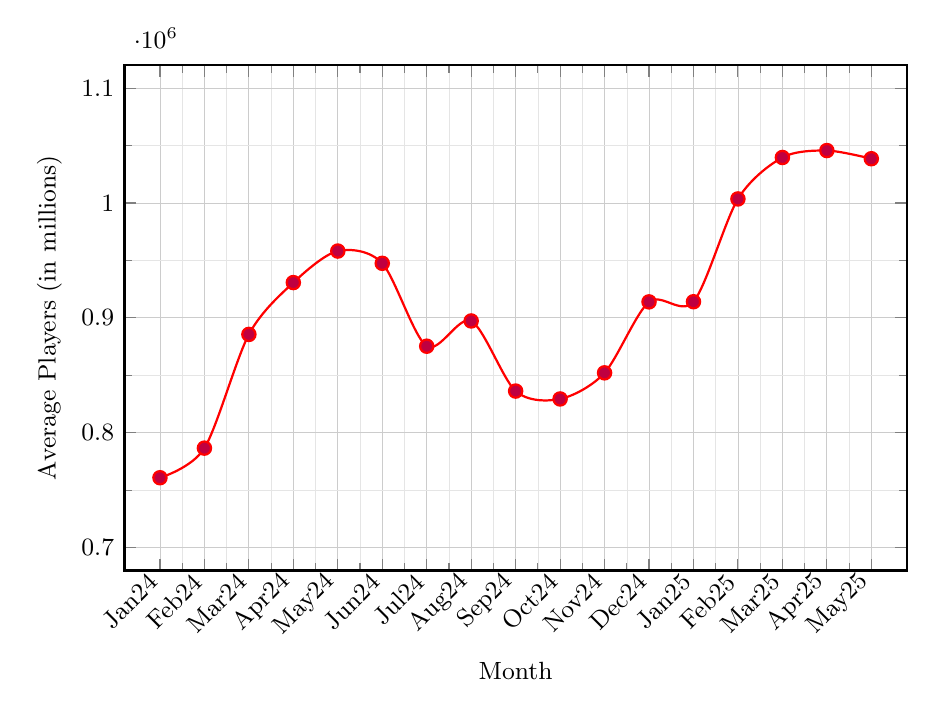
\begin{tikzpicture}
  \begin{axis}[
      width=0.95\textwidth,
      height=8cm,
      xlabel={Month},
      ylabel={Average Players (in millions)},
      symbolic x coords={Jan24, Feb24, Mar24, Apr24, May24, Jun24, Jul24, Aug24, Sep24, Oct24, Nov24, Dec24, Jan25, Feb25, Mar25, Apr25, May25},
      xtick=data,
      xticklabel style={rotate=45, anchor=east, font=\small},
      yticklabel style={font=\small},
      label style={font=\small},
      tick style={thin},
      grid=both,
      minor tick num=1,
      major grid style={line width=.3pt, draw=gray!40},
      minor grid style={line width=.2pt, draw=gray!20},
      ymin=700000, ymax=1100000,
      enlargelimits=0.05,
      smooth,
      mark options={scale=1.2, fill=purple!100},
      line width=0.8pt,
  ]
  \addplot[
      color=red,
      mark=*,
  ]
  coordinates {
      (Jan24,760859) (Feb24,786631) (Mar24,885630) (Apr24,930749)
      (May24,958207) (Jun24,947521) (Jul24,875365) (Aug24,897338)
      (Sep24,836307) (Oct24,829439) (Nov24,852164) (Dec24,913953)
      (Jan25,914092) (Feb25,1003571) (Mar25,1039663) (Apr25,1045702)
      (May25,1038597)
  };
  \end{axis}
  \end{tikzpicture}
  \caption{Evolution of Average CS2 Player Counts (January 2024 to May 2025). Source: SteamCharts.}
  \label{fig:cs2-playerbase}
\end{figure}

The consistent growth in CS2's player base underscores the game's enduring popularity and its pivotal role in the competitive FPS landscape. However, this expansion introduces increased complexity; a larger and more diverse player community amplifies the challenges associated with maintaining competitive integrity.

\newpage

Data from recent enforcement activities further highlights the scale and persistence of the issue \parencite{csstats2024}:

\begin{table}[H]
  \centering
  \small
  \setlength{\tabcolsep}{6pt}
  \caption{Activity of Banned Accounts Prior to Enforcement (January to April 2024)}
  \label{tab:cheater-impact}
  \begin{tabular}{|p{5.2cm}|c|}
  \hline
  \textbf{Metric} & \textbf{Estimated Value} \\
  \hline
  Average delay between last match and VAC ban & 20 days \\
  \hline
  Percentage of bans issued within 24 hours & 28\% \\
  \hline
  Total matches played by banned accounts & Over 32,000 \\
  \hline
  Percentage of matches with only one banned player & 97\% \\
  \hline
  Evidence of case farming behavior & Not significant \\
  \hline
  \end{tabular}
\end{table}

These observations reveal that cheaters are not isolated anomalies; rather, they are embedded within regular matchmaking sessions, further complicating detection and enforcement efforts.

\subsection{Trust Factor and Reporting System Limitations}

To mitigate cheating and enhance matchmaking quality, Valve implemented the \textit{Trust Factor} system in \textit{Counter-Strike 2} (CS2).

\begin{tcolorbox}[colback=gray!10, colframe=gray!50, boxrule=0pt, sharp corners, width=\linewidth, left=1mm, right=1mm, top=0.5mm, bottom=0.5mm]
\makebox[\linewidth][c]{\textbf{Definition: Trust Factor Explained}} \\
The Trust Factor system aggregates multiple indicators such as VAC bans, player reports, account age, and Steam community standing to adjust matchmaking quality. Its opacity aims to prevent manipulation but can lead to confusion and potential exploitation.
\end{tcolorbox}

While the Trust Factor system provides a foundation for fair matchmaking, its lack of transparency presents two significant challenges: (1) players have limited means to understand or improve their Trust Factor; and (2) third-party services offering \textit{report bots} and \textit{commend bots} can manipulate trust metrics for profit \parencite{cs2trustfactor2024}.

\subsection{Economic and Psychological Impact}

The ramifications of cheating extend beyond gameplay, inflicting substantial economic and psychological harm. In early 2025, a significant VAC enforcement wave resulted in the permanent banning of accounts with inventories collectively valued at approximately \$2 million \parencite{escorenews2025vacban}. Although this action was lauded as a crackdown on cheaters, it also raised concerns about transparency and the potential for false positives.

\begin{tcolorbox}[colback=gray!10, colframe=gray!50, boxrule=0pt, sharp corners, width=\linewidth, left=1mm, right=1mm, top=0.5mm, bottom=0.5mm]
\makebox[\linewidth][c]{\textbf{Definition: VAC Ban}} \\
A Valve Anti-Cheat (VAC) ban is a permanent restriction imposed when cheating activity is detected. It disables multiplayer functionality and trading privileges associated with the affected title.
\end{tcolorbox}

For players who have invested considerable time, resources, and personal attachment into their accounts, the psychological toll of encountering cheaters or being wrongfully penalized can be profound, leading to disengagement and a decline in community loyalty.

\section{Community Perception and the Culture of Cynicism}

Cheating incidents are highly visible across social platforms such as Reddit, YouTube, and Twitch. High-profile streamers encountering cheaters during broadcasts exacerbate perceptions of widespread dishonesty, even when empirical cheating rates remain relatively low.

This feedback loop fosters a culture of cynicism, where player trust in matchmaking systems and anti-cheat technologies diminishes, ultimately endangering long-term community stability.

\section{Legal and Ethical Responses to Cheat Development}

Recognizing the limitations of technical interventions, game developers have increasingly turned to legal avenues to combat cheat creators. A notable example is Bungie's legal action against Mihai Claudiu-Florentin, the operator of VeteranCheats, which resulted in a default judgment awarding Bungie \textbf{\$12,059,912.98} in damages. This amount encompassed statutory damages under the Digital Millennium Copyright Act (DMCA), actual damages for copyright infringement, and attorneys' fees and costs \parencite{torrentfreak2023bungie}.

This legal precedent has encouraged other companies, such as Riot Games, Ubisoft, and Activision, to adopt similar strategies in protecting their intellectual property and maintaining fair play within their gaming communities.

\newpage
\section{Anti-Cheat Technologies: Current Trends and Limitations}

Despite significant advancements, contemporary anti-cheat technologies predominantly operate in a reactive capacity, often lagging behind the evolving tactics of cheat developers.

Valve's \textit{Valve Anti-Cheat} (VAC) system primarily employs signature-based detection methods, scanning for known cheat signatures within the game's memory. This approach renders VAC susceptible to evasion techniques such as code obfuscation and manual mapping, which can bypass signature recognition mechanisms \parencite{turn0search0}.

Conversely, Riot Games' \textit{Vanguard} system adopts a more intrusive strategy by operating at the kernel level, granting it deep access to system processes. While this enhances its capability to detect sophisticated cheats, it has raised substantial privacy and security concerns among users due to its persistent presence and high-level system access \parencite{turn0search1}.

Emerging methodologies, including AI-driven behavioral analysis and the utilization of secure enclave technologies, present promising avenues for proactive cheat detection. AI-based systems can analyze player behavior in real-time to identify anomalies indicative of cheating, while secure enclaves offer isolated environments that protect sensitive computations from tampering. However, these approaches introduce new challenges, such as the potential for false positives and concerns regarding user data privacy \parencite{turn0search5, turn0search2}.

The ongoing battle between cheat developers and anti-cheat engineers constitutes a dynamic and relentless arms race, necessitating continuous innovation and adaptation to preserve the integrity of competitive gaming environments.

\vspace{1em}

\begin{tcolorbox}[colback=gray!10, colframe=gray!50, boxrule=0pt, sharp corners, width=\linewidth, left=1mm, right=1mm, top=0.5mm, bottom=0.5mm]
\textbf{Key Takeaways:}
\begin{itemize}
    \item Cheating poses a direct threat to player retention, game reputation, and revenue streams.
    \item Systems like \textit{Trust Factor} require increased transparency and user engagement to be effective.
    \item Legal actions are a critical component in combating organized cheat development and distribution.
    \item The fight against cheating is an ongoing, adaptive arms race necessitating continual technological and strategic innovation.
\end{itemize}
\end{tcolorbox}
